%==========================================================
\section{Interface de utilizador}\label{sec:interface}

Para a nossa interface, nós temos dois claros focos: o jovem cliente e o agente.
Nós supomos que o jovem cliente utiliza a versão base do nosso sistema Roamly, enquanto o agente utiliza a versão premium.
Para cada ponto de foco, temos 3 janelas que apresentam as funcionalidades principais do sistema.
Para fazer login, assumimos que uma janela para esse efeito aparecerá após a aplicação ser iniciada.
Para utilizadores com a versão base, login não é necessário.
Para fazer logout, basta clicar no nome do utilizador (que nas janelas do agente é "Agente C") para que um menu apareça, onde se possa fazer logout.

\subsection{Wireframes}

\begin{figure}[!ht]
  \centering
  % Pair 1
  \begin{subfigure}{0.45\textwidth}
    \centering
    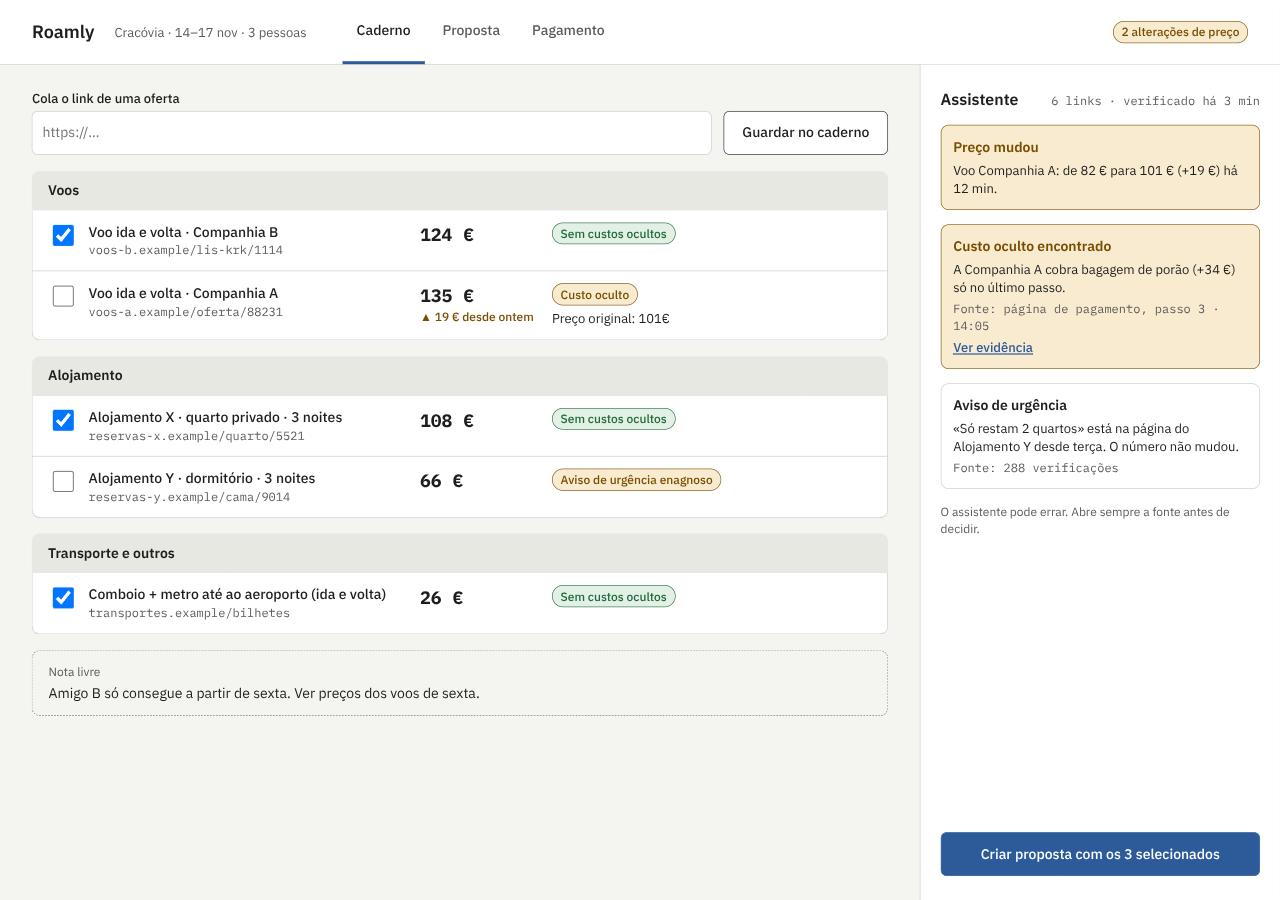
\includegraphics[width=\linewidth]{figuras/jovem1.png}
    \caption{Caderno de ofertas do Jovem}
  \end{subfigure}\hfill
  \begin{subfigure}{0.45\textwidth}
    \centering
    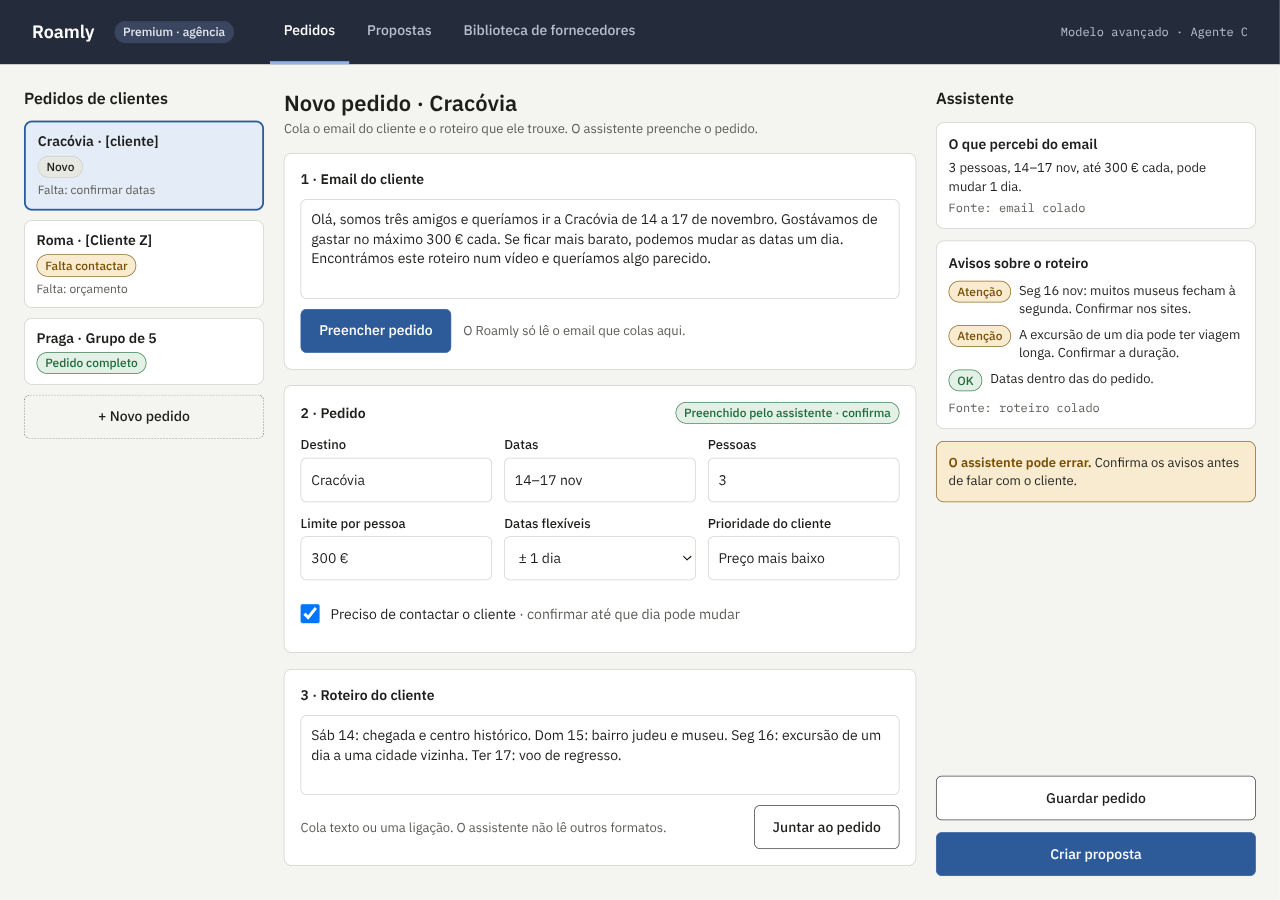
\includegraphics[width=\linewidth]{figuras/agente1.png}
    \caption{Pedidos dos clientes do Agente}
  \end{subfigure}\hfill
  \begin{subfigure}{0.45\textwidth}
    \centering
    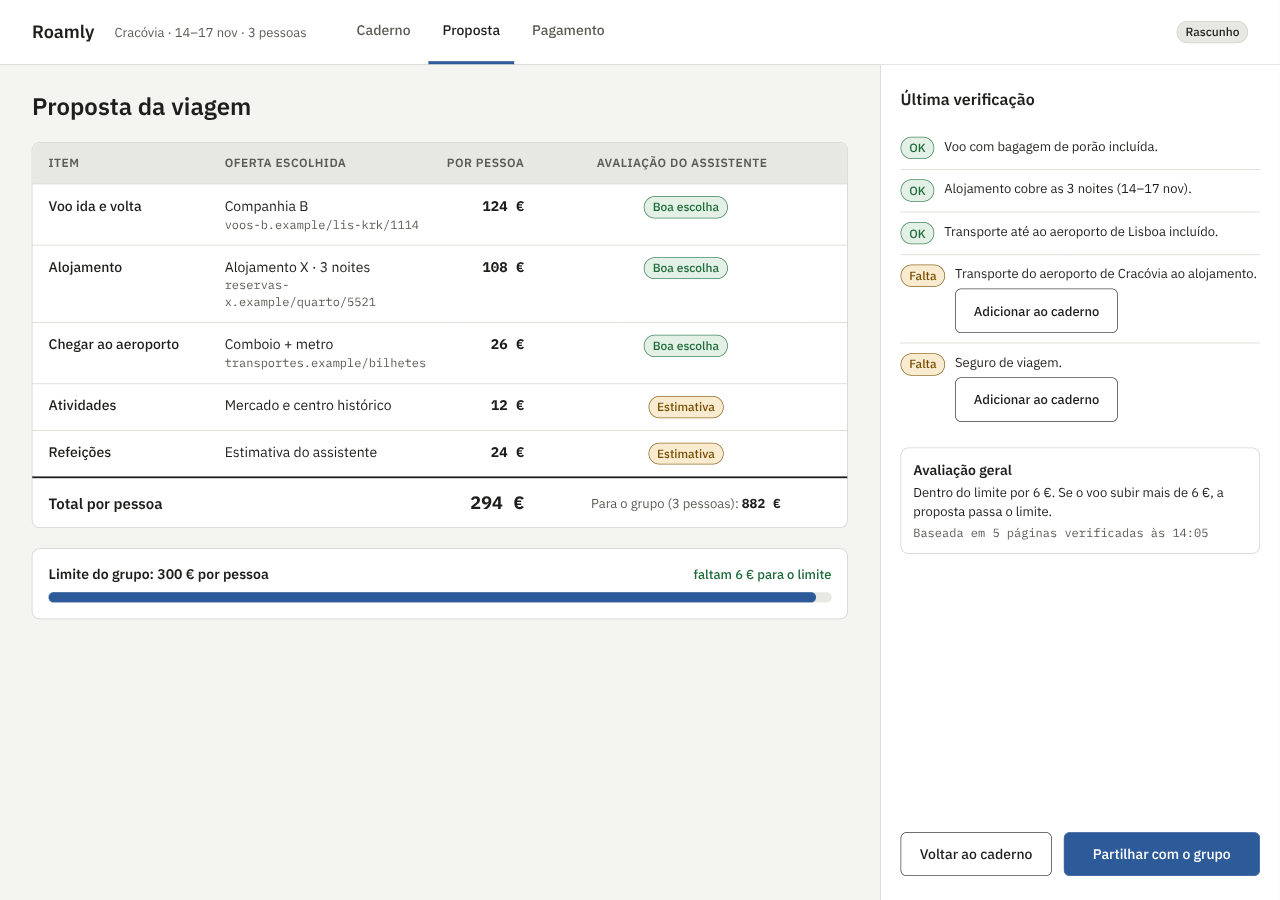
\includegraphics[width=\linewidth]{figuras/jovem2.png}
    \caption{Proposta de viagem do Jovem}
  \end{subfigure}\hfill
  \begin{subfigure}{0.45\textwidth}
    \centering
    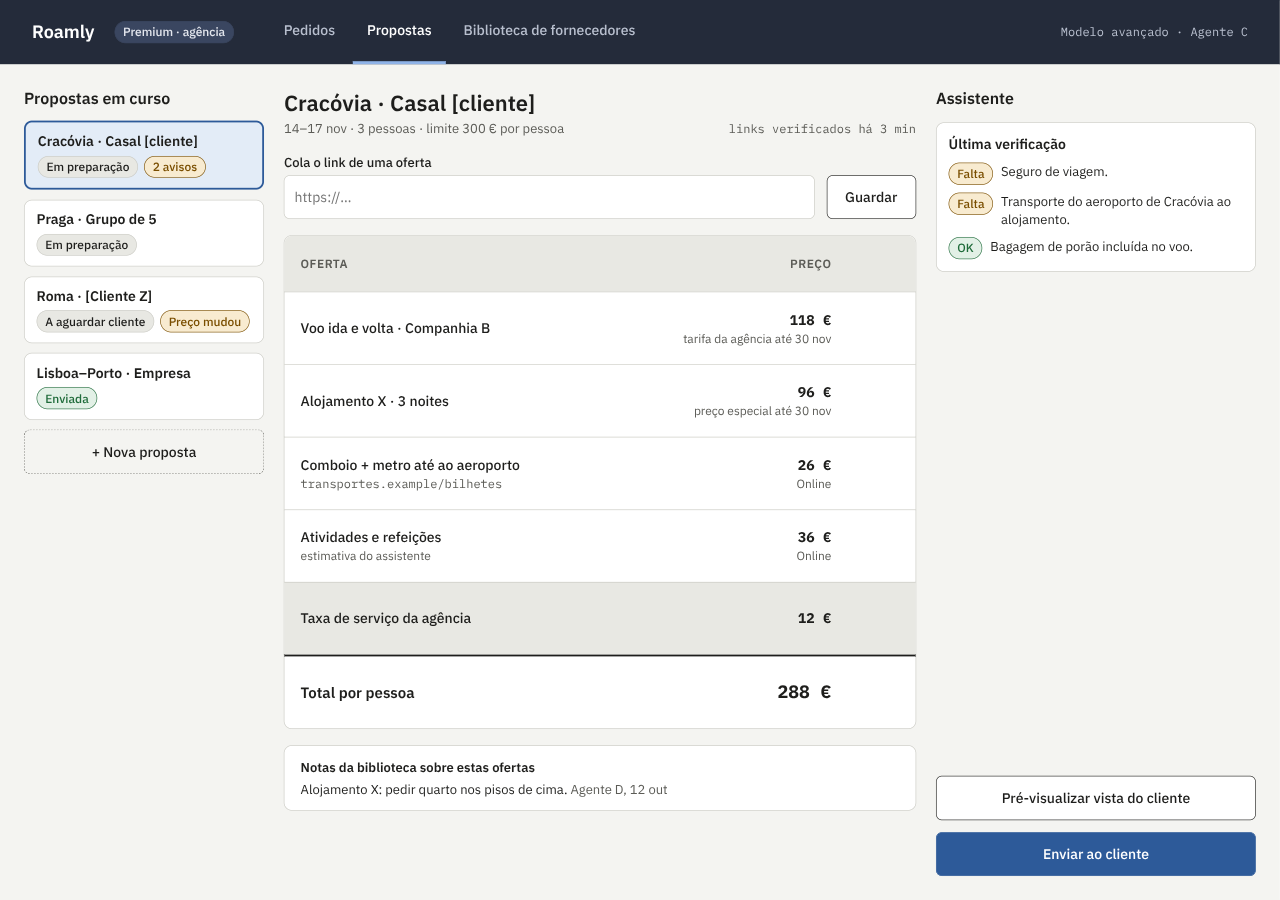
\includegraphics[width=\linewidth]{figuras/agente2.png}
    \caption{Proposta de viagem de um cliente do Agente}
  \end{subfigure}\hfill
  \begin{subfigure}{0.45\textwidth}
    \centering
    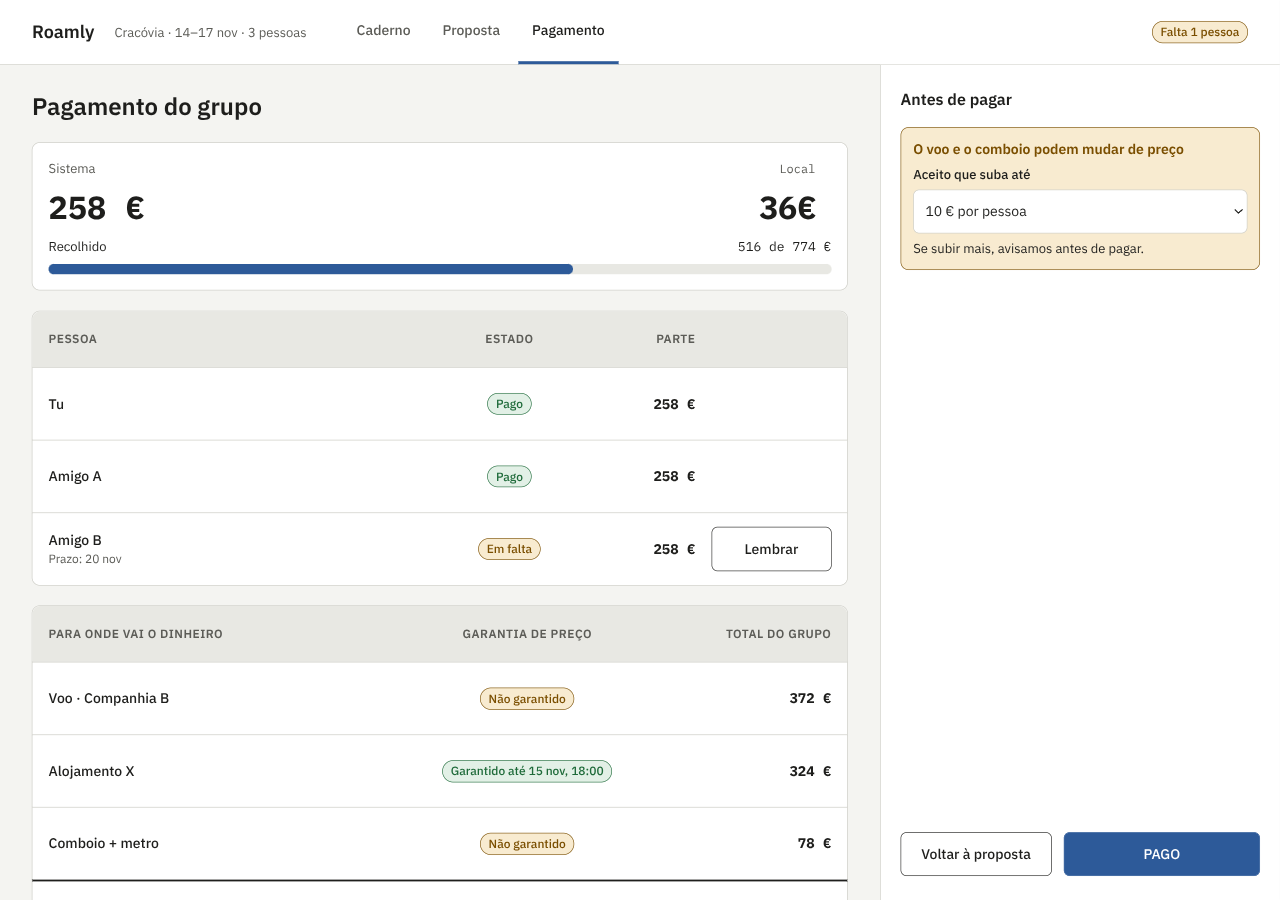
\includegraphics[width=\linewidth]{figuras/jovem3.png}
    \caption{Pagamento do Jovem e dos seus colegas}
  \end{subfigure}\hfill
  \begin{subfigure}{0.45\textwidth}
    \centering
    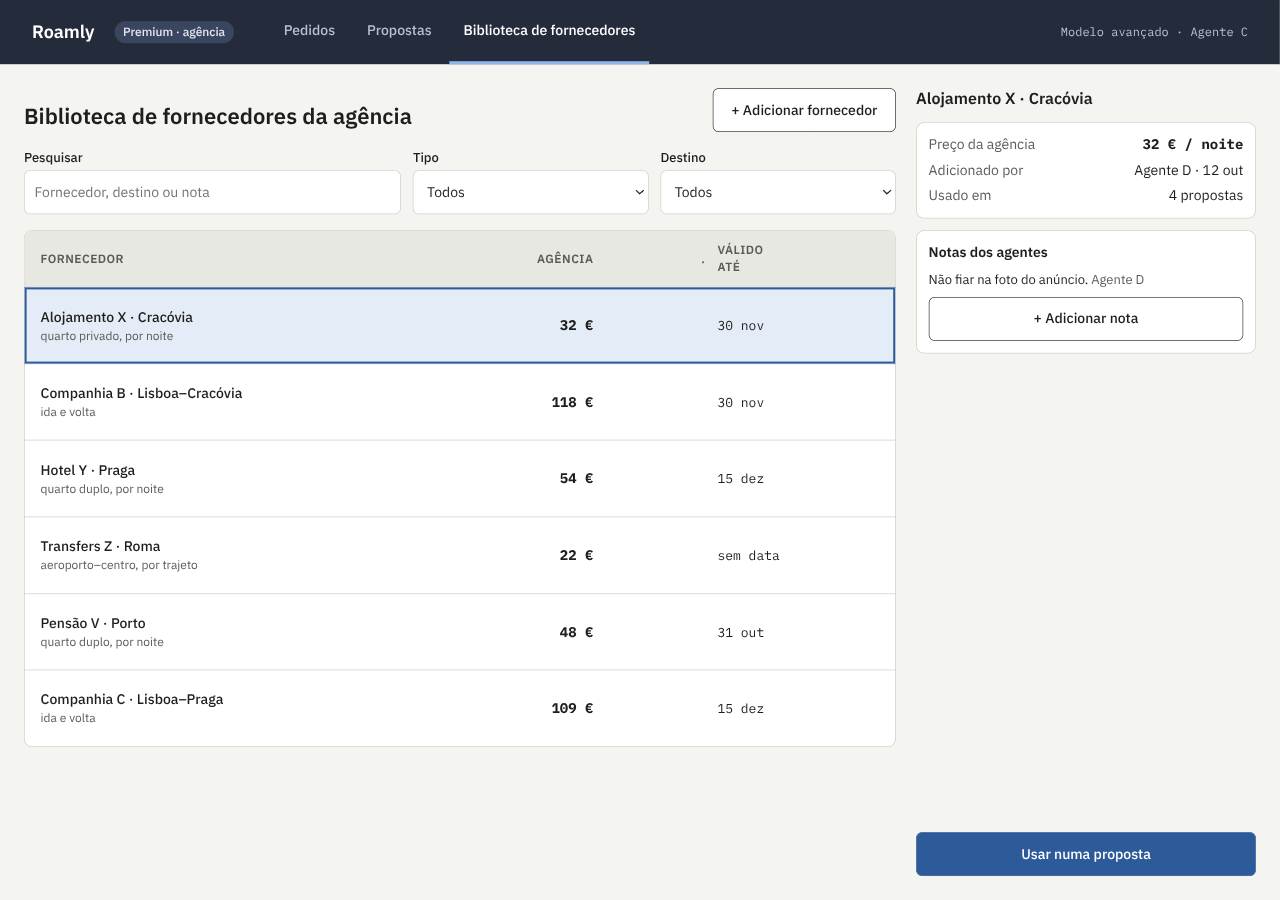
\includegraphics[width=\linewidth]{figuras/agente3.png}
    \caption{Biblioteca de fornecedores do Agente}
  \end{subfigure}\hfill
  \caption{6 janelas da nossa interface de utilizador. À esquerda, para o Jovem. À direite, para o Agente}
  \label{fig:three_pairs}
\end{figure}

\subsection{Avaliação de usabilidade de Nielsen}